% -*- mode : latex; coding: utf-8 -*-
\chapter{Background} \label{sec:Backgrounds}

\section{DRAM Overview}
\subsection{DRAM Organization}

\begin{figure}[ht]
  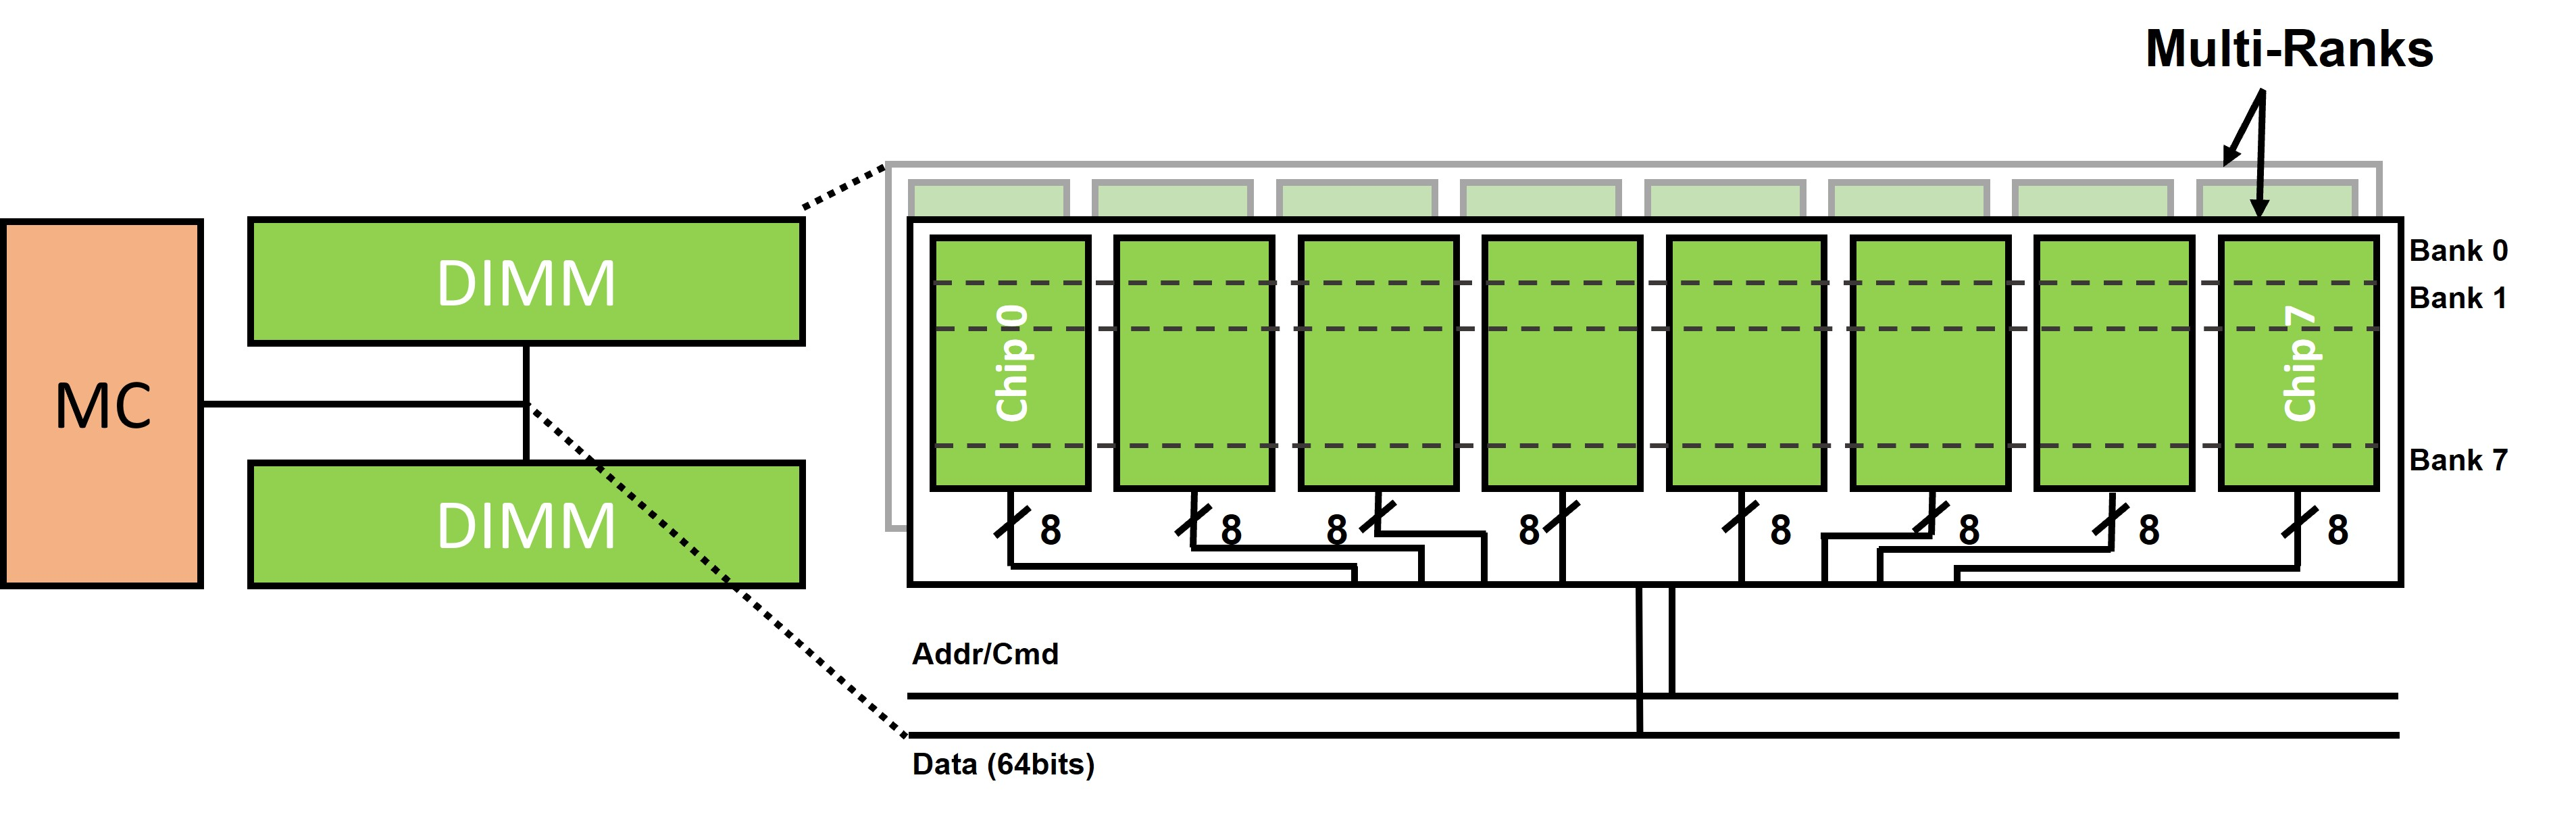
\includegraphics[width=\textwidth]{figures/DDR system overview.jpg}
  \caption{Overview of DDR memory system}
\label{fig:DDR_overview}
\end{figure}

Typical DDR memory systems consist of multiple memory controllers (MCs). 
Single MC controls channel(s) and each channel consist of single or multiple ranks 
(See Figure \ref{fig:DDR_overview}), where several DRAM devices (chips) operate in lock-step.  
Each DRAM chip accepts the address with the command and outputs data in the DQ pin. 
Several independent banks reside in each chip, and adjacent data is interleaved into different banks in order to 
hide memory access latency. 

\begin{figure}[ht]
  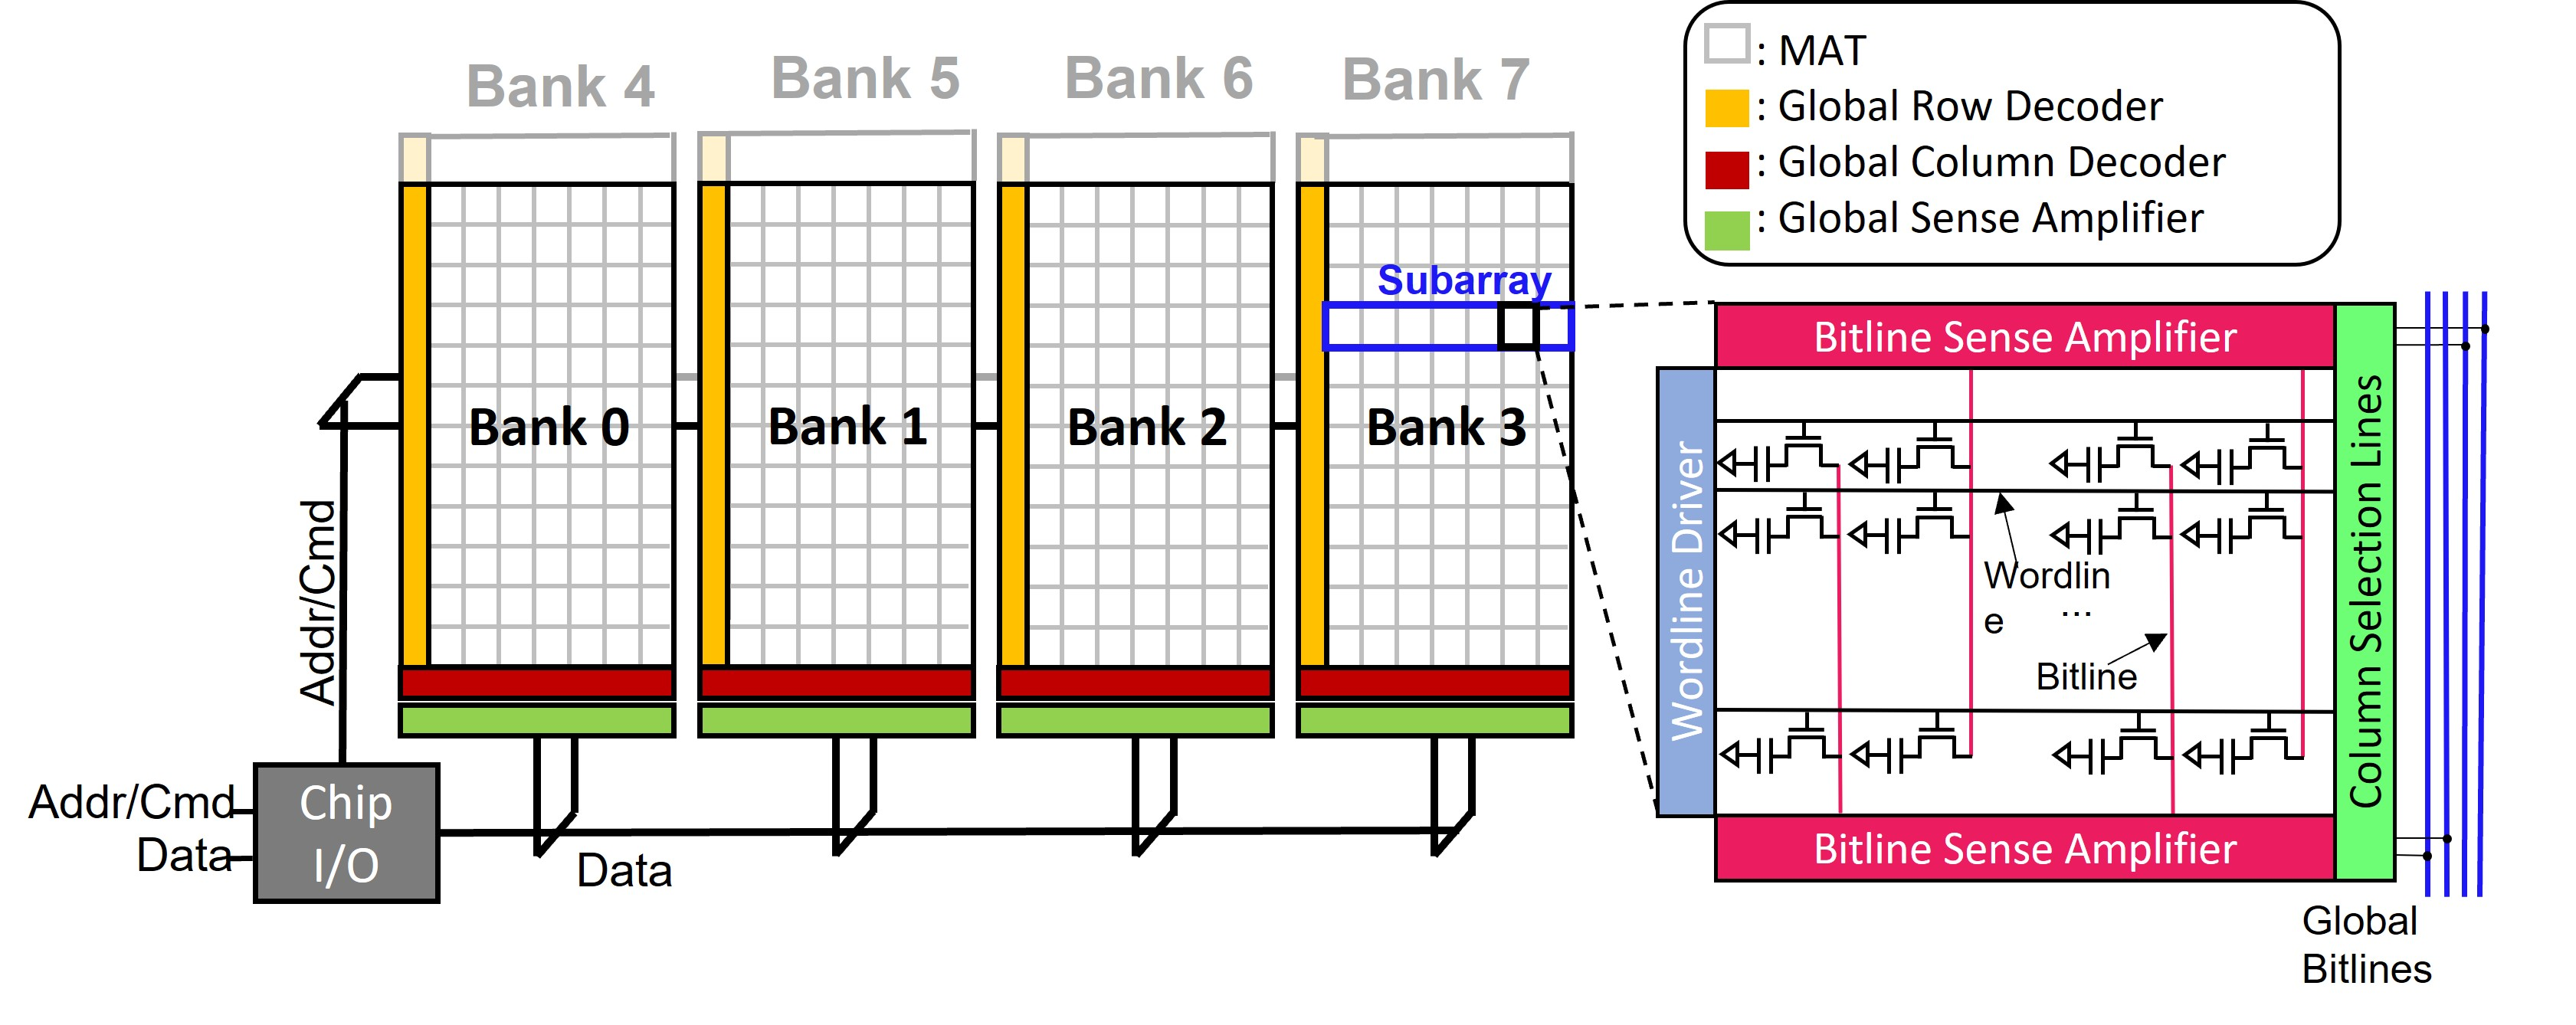
\includegraphics[width=\textwidth]{figures/DRAM chip.jpg}
  \caption{DRAM chip organization}
\label{fig:DRAM_chip}
\end{figure}

Figure \ref{fig:DRAM_chip} shows the hierarchy inside a DRAM chip. Chip has several banks, and each bank 
consists of multiple MATs. MAT is a matrix of cells (typically 512$\times$512 or 1024$\times$1024) each connected by 
wordline (WL) and bitline (BL). MATs sharing local sense amplifiers form subarray. When a row address comes to the global 
row decoder, it selects the subarray row decoder which in turn activates WL (i.e. target address) via wordline drivers. 
When local WL is activated, data in each cell is read from BL to a local sense amplifier. 
Since each sense amplifier is much larger than each cell, putting sense amplifiers in one place can make a composition of cells inside MATs 
sparse. Since sense amplifier is symmetric, it can be connected at top of MAT as well as the bottom. 
This architecture is called \textit{open bitline architecture} and can lead to a more compact design of MATs. After data is read to a local 
sense amplifier, a column select line chooses data corresponding to the column address and the data is sent to the global sense amplifier 
by global bitlines. 
\subsection{Timing}
Due to the master-slave interface between MC and DRAM device, MC has to be stalled for a predefined amount of time between each
command. Also, the capacitor in the DRAM cell slowly leaks when idle. The amount of time a DRAM cell can retain its
data is called \textit{retention time}. MC prevents cells from losing their data by periodically sending a restore
command which is called \textit{refresh}. DDR4 standard \cite{JEDEC_DDR4} specifies timing parameters related to the refresh command,
which is the refresh interval. Refresh interval ($\mathbf{tREFI}$) is a period of refresh command sent to DRAM to refresh DRAM row 
(or group of rows). In order to preserve data, the refresh period for a given row ($\mathbf{tREFW}$) must be shorter than the minimum retention time for entire cells in DRAM. This parameter is vendor-specific, and the JEDEC standard does not specify tREFW. 
Typical values of tREFW, tREFI, and other timing parameters for DRAM read/write are summarized in table \ref{tab:DDR4_timing}.

\begin{table}[t]
  \centering
  \caption{Typical DDR4 timing parameters used in paper}
  \label{tab:DDR4_timing}
  \begin{tabular}{llr}
  \toprule
    Term  &  Definition & Value \\
  \midrule 
    tREFI & Refresh period & 7.8$\mu$s \\ 
    tREFW & Refresh period for single row & 64ms \\
    tRFC & Refresh command duration & 350ns  \\ 
    tRC & Row cycle time & 45ns  \\
  \bottomrule
  \end{tabular}
  \vspace{-0.20in}
\end{table}

\section{RowHammer}
\subsection{Phenomenon}
Repetitive activation of a single row makes a small number of electrons flow at adjacent cells, making its cells discharge faster. 
This causes bits to be flipped, enabling an attacker to manipulate data without accessing them. Rows repetitively accessed
to cause bitflip is called \textit{aggressor rows}, and rows affected by aggressor rows are called \textit{victim rows}. 
A minimum number of ACT commands required to induce bitflip is called $Flip_{th}$. 
Since $Flip_{th}$ is getting lower due to technology scaling in DRAM, finding an efficient solution is becoming more important.

\subsection{Existing Solutions and Limitations}
\label{sec:Existing Solutions}
Numerous solutions have been proposed by both academia and industry. Recent researches focus on architectural scheme,
which implements hardware logic inside MC or DRAM (or both) to detect aggressor rows at run time and handle them. 
PARA \cite{FlippingBits}, a probabilistic approach to refresh adjacent rows with small predefined probability, doesn't
require complex tracking logic but suffers from a significant amount of unnecessary refresh which degrades performance
seriously. Counter-based approach, on the other hand, reserve counter for aggressor rows and refreshes victim rows
when the counter reaches a predefined threshold. TWiCe \cite{TWICE} proposed \textit{Near Row Refresh} (NRR) command for
handling such victim refresh: When MC sends NRR, the DRAM device finds and refreshes two adjacent rows of
the command. There are two inefficiencies in this approach. First, MC doesn’t know which physical row corresponds to a given logical row, 
so the tracker must assume the most malicious kinds of attack: a single victim row between two aggressor rows (double-sided). 
Thus, the bitflip threshold is halved. Second, when the bitflip threshold is reached, MC just sends the NRR command without feedback 
from the DRAM chip. So MC doesn’t know which rows were refreshed, enabling attackers to utilize migitation action itself for an attack: 
Half-double \cite{Half_Double}. Below I present two state-of-the-art counter-based approaches and their limitations.

\begin{figure}[ht]
  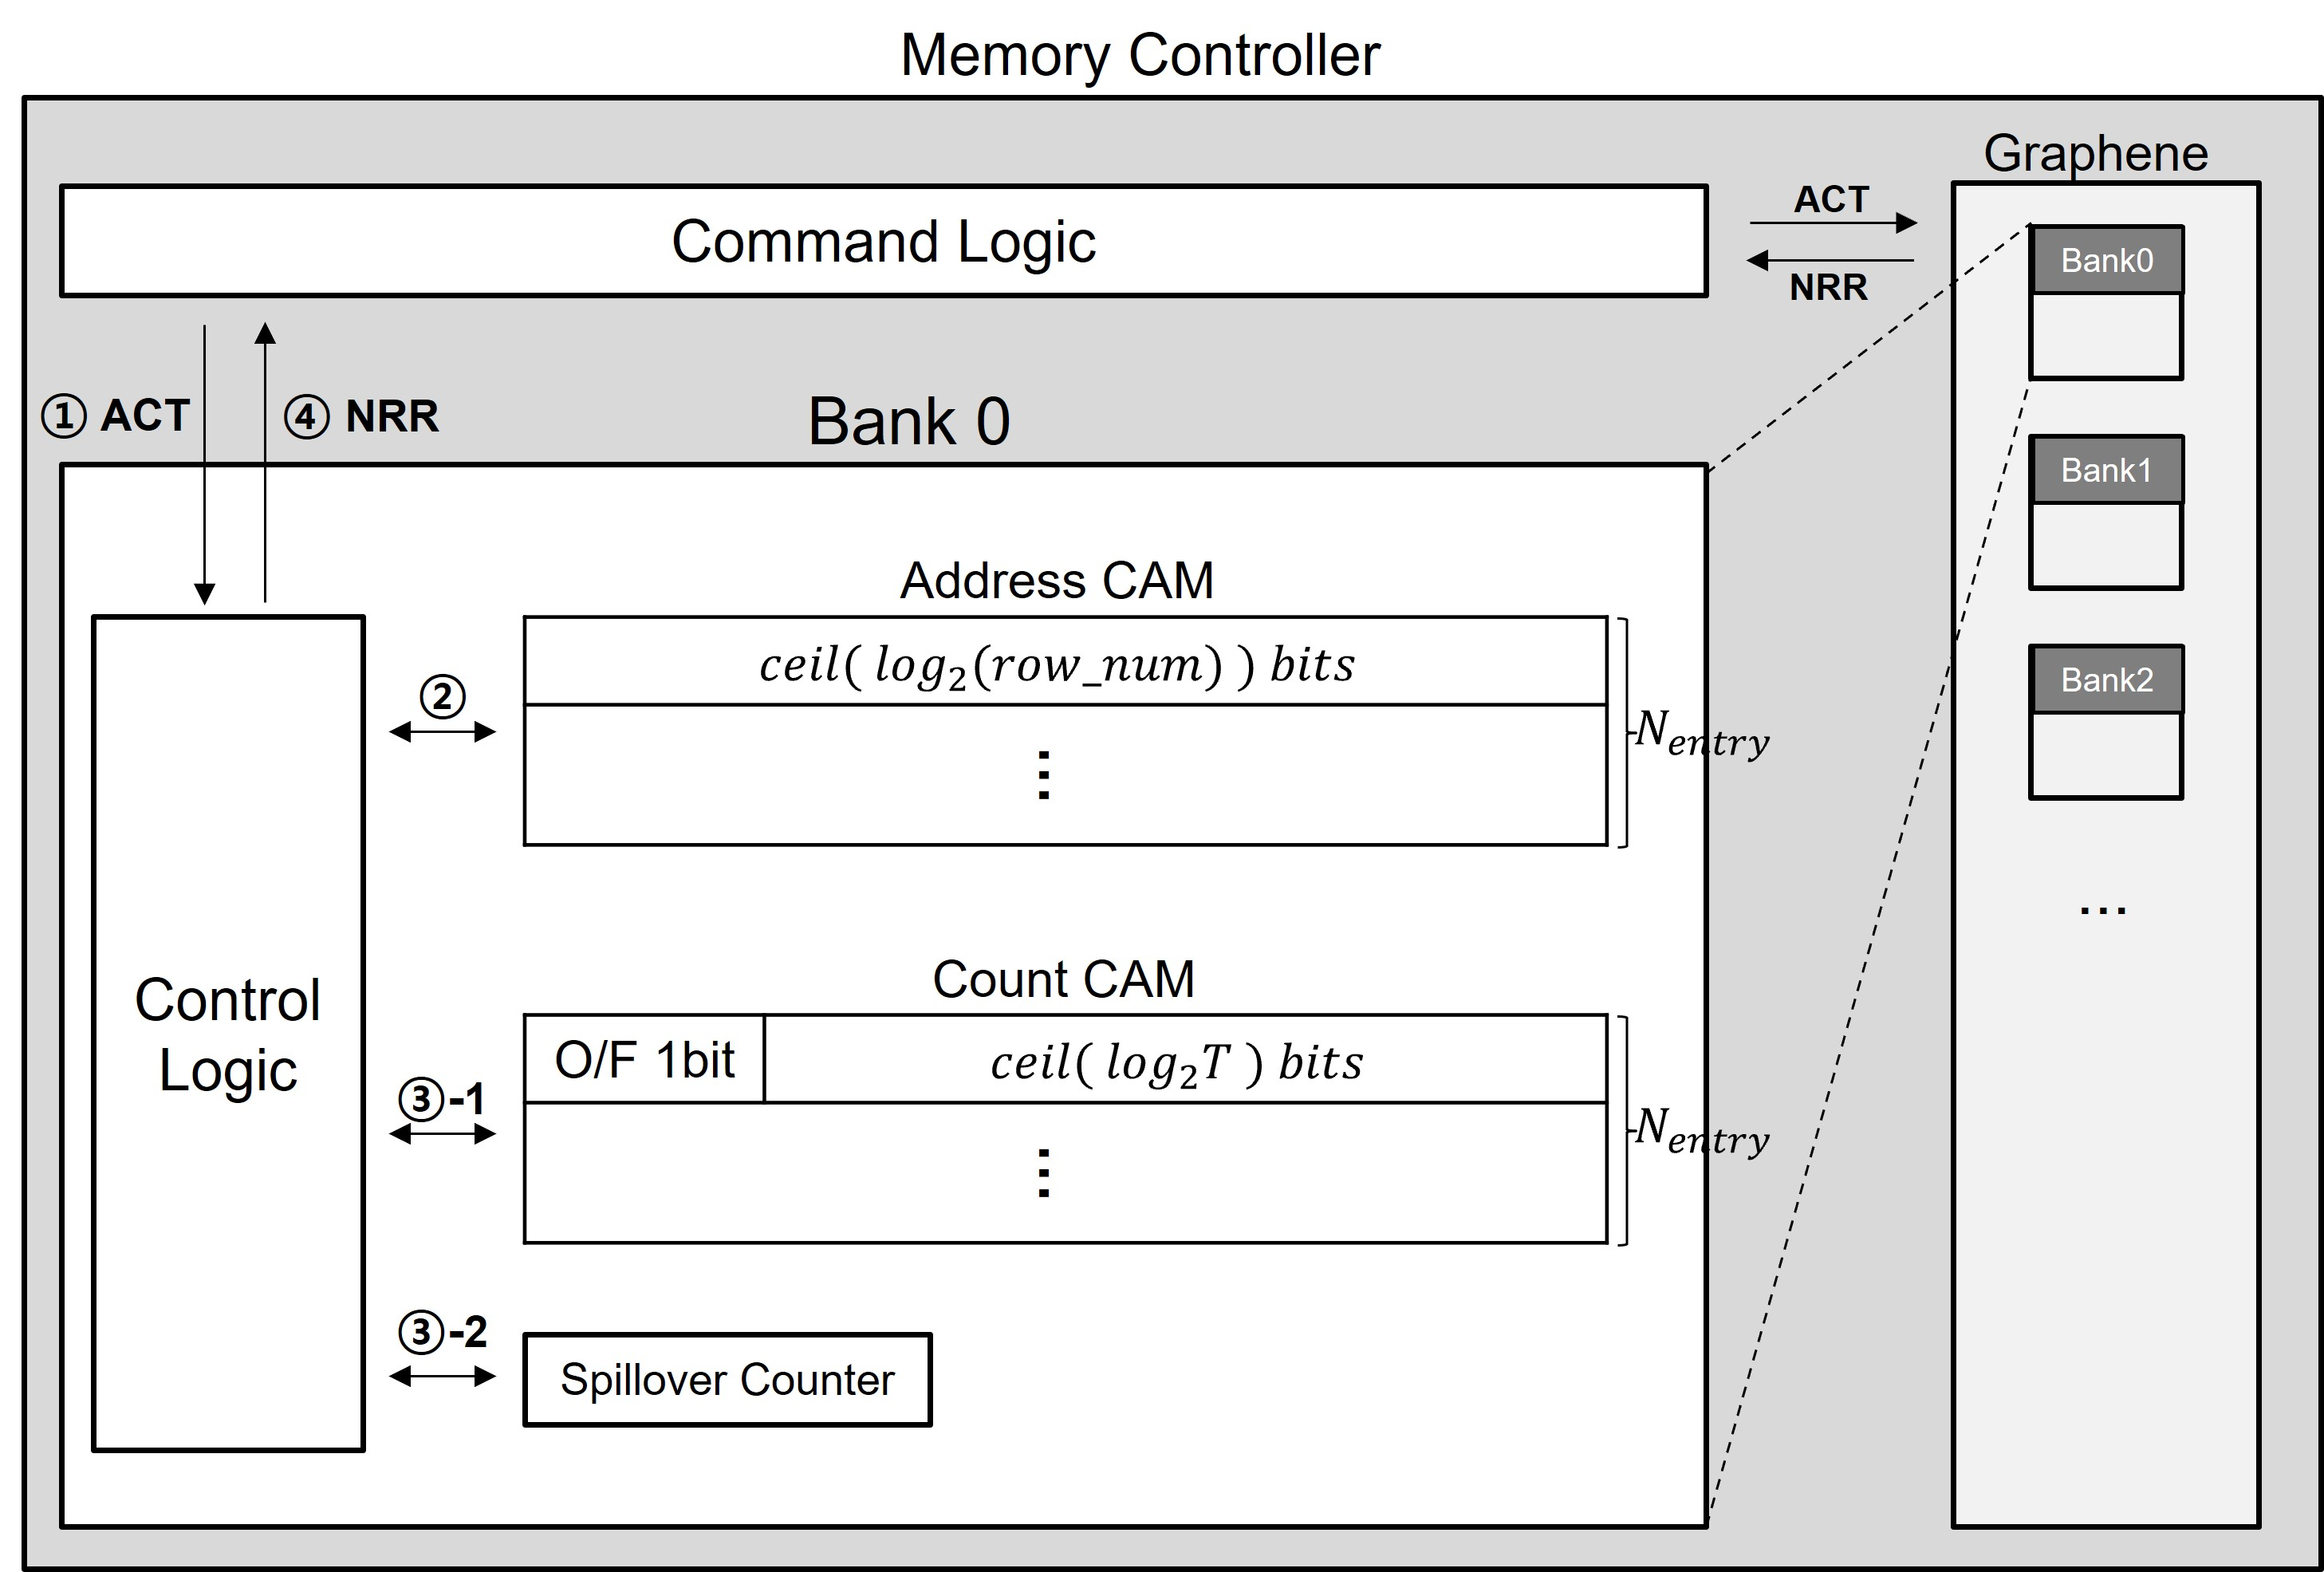
\includegraphics[width=\textwidth]{figures/Graphene.jpg}
  \caption{Graphene Overview}
\label{fig:Graphene}
\end{figure}

\noindent\textbf{Graphene} utilizes the Misra-Gries algorithm \cite{MISRA-GRIES} to track the number of ACTs each row received
during tREFW. Figure \ref{fig:Graphene} shows an overview of Graphene. It maintains counter CAM for incoming 
ACTs in MC per each bank. \raisebox{.5pt}{\textcircled{\raisebox{-.9pt} {1}}} ACTs goes into corresponding bank, 
and \raisebox{.5pt}{\textcircled{\raisebox{-.9pt} {2}}} consults its address CAM.
In case of hit (\raisebox{.5pt}{\textcircled{\raisebox{-.9pt} {3}}} -1), it accesses count CAM and increments the counter by 1. 
If the entry is not in count CAM, it then checks if any entry in count CAM has the same value
as the spillover counter (\raisebox{.5pt}{\textcircled{\raisebox{-.9pt} {3}}}-2). If an entry is found, it evicts it and increments a counter.
If not found, it increments the spillover counter. If the incremented counter matches the predefined threshold T (\raisebox{.5pt}
{\textcircled{\raisebox{-.9pt} {4}}}-2), Graphene control logic sends out an NRR command. 
Although simple and intuitive, MC must assume that every attack is double-sided 
and T is half of $Flip_{th}$. Due to the steady trend of decreasing $Flip_{th}$, T is also decreased, 
which makes $N_{entry}$ bigger. This leads to a bigger, slower Count CAM.

\begin{figure}[ht]
  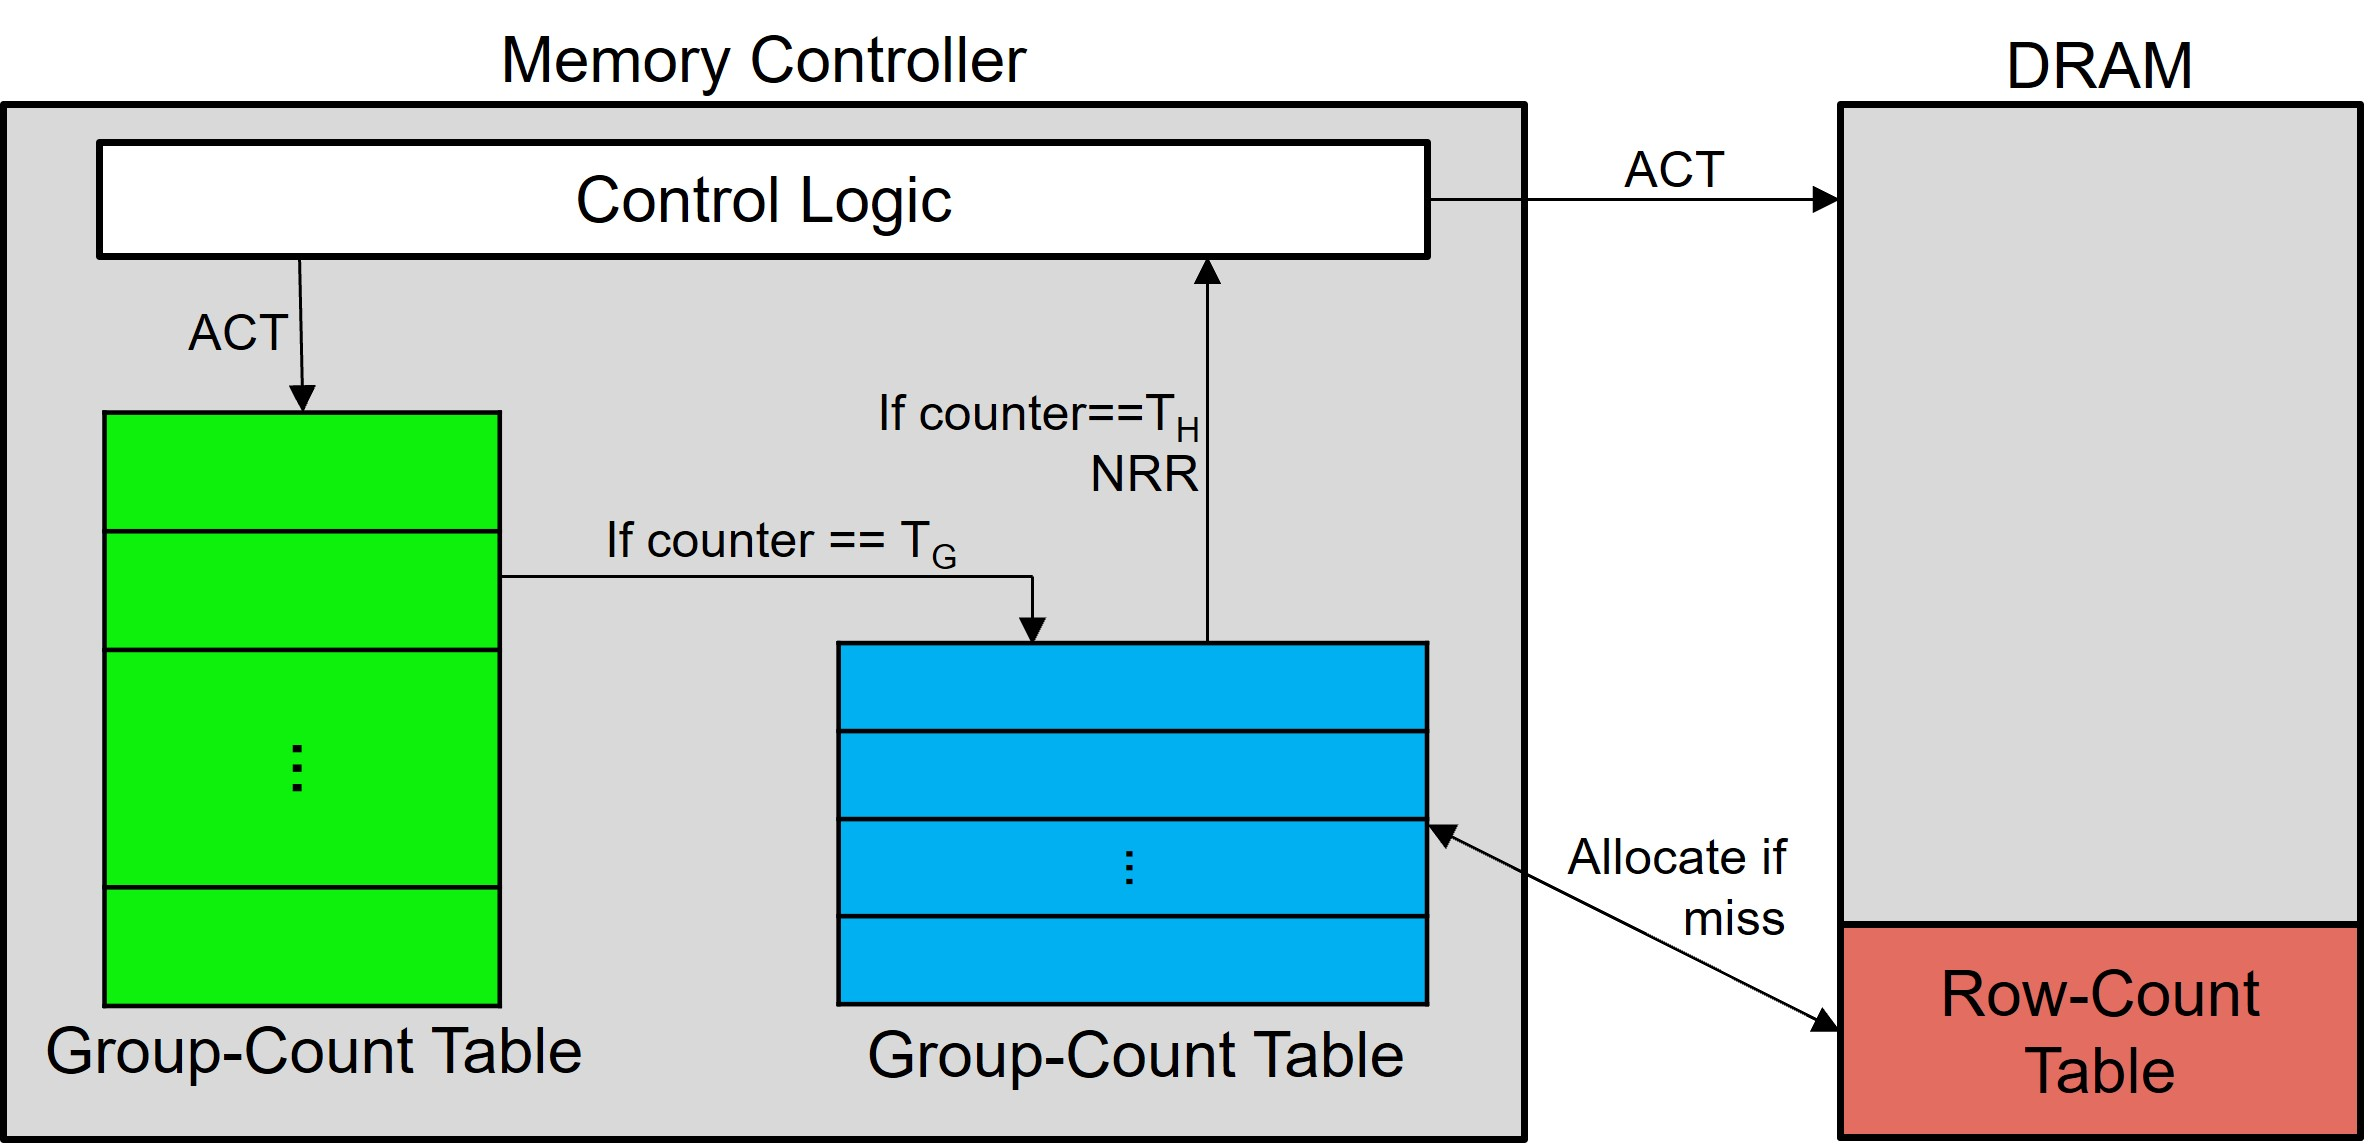
\includegraphics[width=\textwidth]{figures/Hydra.jpg}
  \caption{Hydra Overview}
\label{fig:Hydra}
\end{figure}

\noindent\textbf{Hydra} is a counter-based mitigation scheme targeting low $Flip_{th}$ with small storage overhead. 
It uses a hybrid scheme of two counter tables each with a predefined threshold: SRAM Group-Count Table (GCT) with $T_{G}$ 
and DRAM Row-Count Table with $T_{H}$. GCT is an SRAM counter indexed by row address which is used to filter non-malicious attacks. 
All rows are statically mapped to a single entry in GCT, forming a \textit{Row-Group}. RCT is a predefined region inside DRAM that saves 
counters for each row. Counters are untagged and can record values up to $T_{H}$. Figure \ref{fig:Hydra} shows a high-level overview
of Hydra. At run time, each GCT entry stores aggregated activation count of corresponding row-group. 
When GCT entry reaches $T_{G}$, Hydra switches from group counting to per-row counting for rows in the group. 
All counters for row-group are initialized as $T_{G}$, and all subsequent access of rows in the group goes into RCT instead of GCT. 
When the RCT counter reaches $T_{H}$, Hydra control logic sends out an NRR command. 
To reduce the performance overhead of extra DRAM access when updating the RCT counter, 
Hydra used Row-Count Cache (RCC) to cache each frequently accessed RCT entry. 
Although this scheme scales well with decreasing $Flip_{th}$, it uses the same NRR-based mitigation as Graphene
which leads to the halved threshold and possible security breakage. 
